
\chapter{Θεωρητική Ανάλυση και Αλγόριθμοι} % Main chapter title

\label{Θεωριτική Ανάληση} % Change X to a consecutive number; for referencing this chapter elsewhere, use \ref{ChapterX}

\lhead{Κεφάλαιο 2. \emph{Θεωρητική Ανάλυση}} % Change X to a consecutive number; this is for the header on each page - perhaps a shortened title


%----------------------------------------------------------------------------------------
%	SECTION 1
%----------------------------------------------------------------------------------------


\section{Προσωποποίηση}
\noindent
Η βασική φιλοσοφία ενός συστήματος Προσωποποίησης είναι \emph{να παρέχει στους χρήστες
τις πληροφορίες που θέλουν ή χρειάζονται, χωρίς να περιμένει να του ζητηθεί ρητά}.\cite{mulvenna2000personalization}\\
Τα δομικά στοιχεία της προσωποποίησης των δικτύων είναι:\\
- Η κατηγοριοποίηση και προεπεξεργασία των δεδομένων.\\
- H εξόρυξη των συσχετίσεων μεταξύ διαφορετικών ειδών δεδομένων.\\
- Ο προσδιορισμός των ενεργειών που θα προταθούν από το σύστημα.\cite{mobasher2000automatic}\\
Ο πιο διαδεδομένος τρόπος επίτευξης της προσωποποίησης είναι με την εφαρμογή ενός Συστήματος Συστάσεων. 
\cite{eirinaki2003web}



\section{Συστήματα Συστάσεων}
\noindent
Ένα \emph{Σύστημα Συστάσεων (Recommender System)} είναι ουσιαστικά ένας μηχανισμός που
ως πρώτο σκοπό έχει το να προβλέψει το ενδιαφέρον ενός χρήστη για αντικείμενα με τα 
οποία δεν έχει ακόμα επαφή.
Εντοπίζοντας και εμφανίζοντας στο χρήστη αντικείμενα με μέγιστο εκτιμώμενο ενδιαφέρον,
επιτυγχάνεται η προσωποποίηση μιας Web υπηρεσίας και ο χρήστης καταφέρνει να αποφύγει την υπερπληροφόρηση έχοντας πρόσβαση σε ένα υποσύνολο των αντικειμένων
της υπηρεσίας το οποίο τον ενδιαφέρει περισσότερο σύμφωνα με τις μέχρι στιγμής προτιμήσεις του.
Σε αυτήν την παράγραφο θα επιχειρήσουμε μία εισαγωγή στα Recommender Systems (συστήματα συστάσεων) και στις υπάρχουσες θεωρητικές και πρακτικές κατευθύνσεις. 
  
\subsection{Εισαγωγή Στα Συστήματα Συστάσεων}
\noindent
Στη μελέτη επισκόπησης των \emph{Adomavicius} και \setlanguage{english}  \emph{Tuzhilin} \cite{NGRS} \setlanguage{greek} όπου πραγματοποιήθηκε έρευνα σχετικά με το υπάρχον στάδιο 
των \setlanguage{english} Recommender systems, \setlanguage{greek} αντλήθηκαν και παρουσιάζονται τα παρακάτω στοιχεία.
  
Τα συστήματα συστάσεων αναδύθηκαν σαν ερευνητικό πεδίο μετά την εμφάνιση των πρώτων papers σχετικών με το collaborative filtering στα μέσα της δεκαετίας του 90. 
Τόσο στην ακαδημαϊκή κοινότητα αλλά και στον επιχειρηματικό κόσμο, την τελευταία δεκαετία, γίνονται προσπάθειες εύρεση και υλοποίηση νέων προσεγγίσεων. 
Το ενδιαφέρον παραμένει ακόμα υψηλό καθώς υπάρχουν πολλά ακόμα προβλήματα προς επίλυση και χώρος για την ανάπτυξη προσωποποιημένων εφαρμογών, καθώς οι χρήστες των διαδικτυακών
υπηρεσιών καλούνται να αντιμετωπίσουν την ολοένα και μεγαλύτερη υπερπληροφόρηση.

Σχετικές έννοιες είχαν ήδη αναφερθεί σε διαφορετικούς τομείς όπως στην ανάκτηση 
πληροφορίας \setlanguage{english}(information retrieval)\setlanguage{greek} 
αλλά και στο μάρκετινγκ,
αποτέλεσε όμως ανεξάρτητο πεδίο από την στιγμή που οι ερευνητές άρχισαν να μελετούν 
\emph{προβλήματα βαθμονόμησης \setlanguage{english} (ranking problems)}\setlanguage{greek} 
των συστάσεων. 
Ο πυρήνας ενός Συστήματος Συστάσεων είναι ουσιαστικά μια διαδικασία πρόβλεψης
αξιολογήσεων(rating) των αντικειμένων με τα οποία ο χρήστης δεν είχε ακόμα επαφή,
και στη συνέχεια βαθμονόμησης των αντικειμένων με βάση την αξιολόγηση,
ώστε τελικά να προταθούν στον χρήστη τα αντικείμενα με την υψηλότερη εκτιμώμενη αξιολόγηση.\\

Αν επιχειρήσουμε μια πιο τυπική διατύπωση των παραπάνω έχουμε:\\
Ένα σύνολο χρηστών $C$ και ένα σύνολο αντικειμένων $S$. \\
Επίσης έχουμε $u$ τη συνάρτηση χρησιμότητας ενός αντικειμένου $s$ για τον χρήστη $c$.
Τότε για τη συνάρτηση χρησιμότητας $u$ ισχύει ότι 

$u:C$x$S \rightarrow R$,  με R να είναι ένα καθορισμένο σύνολο (π.χ. μη αρνητικοί ακέραιοι ή πραγματικοί αριθμοί κάποιου εύρους).

Στην συνέχεια για κάθε χρήστη $c\in C$, θέλουμε να επιλέξουμε κάποιο αντικείμενο $\acute{s}\in S$ το οποίο να μεγιστοποιεί 
το εκτιμώμενο ενδιαφέρον (\emph{χρησιμότητα}) του χρήστη για αυτό.

Επομένως:   $\forall c\in C,  \acute{s_c}=\arg_{s\in S} \max u(c,s) $   

Συνήθως στα συστήματα συστάσεων η χρησιμότητα ενός αντικειμένου εκφράζεται με μια αξιολόγηση, εναλλακτικά η χρησιμότητα μπορεί να προκύπτει από μια καθορισμένη συνάρτηση κέρδους.
Ανάλογα με την φύση της εφαρμογής, η χρησιμότητα $u$ μπορεί είτε να δηλωθεί από τον χρήστη με την μορφή αξιολόγησης,
είτε να υπολογιστεί από την ίδια την εφαρμογή όπως στην περίπτωση της συνάρτησης κέρδους.

Κάθε μέλος του συνόλου χρηστών $C$ περιγράφεται από ένα \emph{προφίλ (userProfile)} που περιλαμβάνει προσωπικές πληροφορίες, όπως δημογραφικά στοιχεία ή προτιμήσεις.
Στην πιο απλή περίπτωση μοναδικό στοιχείο που χρειάζεται είναι ένα userID. 
Παρομοίως κάθε στοιχείο του συνόλου των αντικειμένων $S$ μπορεί να περιγράφεται από ένα σύνολο χαρακτηριστικών. 
\cite{NGRS}

\subsection{Μέθοδοι Συστάσεων}
\noindent
Hill, Resnick και Shardanand είναι μερικοί από τους θεμελιωτές 
της σύνθεσης κοινώς αποδεκτών μεθόδων για την παραγωγή συστάσεων.
\cite{hill1995recommending} \cite{resnick1994grouplens} \cite{shardanand1995social}\\
Έκτοτε το πρόβλημα έλαβε τις υπάρχουσες διαστάσεις του και άρχισε να μελετάται περαιτέρω.
  
Τα Συστήματα Συστάσεων υπάγονται στις ακόλουθες γενικές κατηγορίες ανάλογα με τον τρόπο προσέγγισης των αξιολογήσεων:

\begin{description}
\item \textbf{Content-based recommendations}  \hfill \\
Η πρόβλεψη των αξιολογήσεων προκύπτει από τις αξιολογήσεις που έχει κάνει ο χρήσης σε άλλα αντικείμενα. 
Επομένως τελικά προτείνονται αντικείμενα παρόμοια με αυτά που έχει αξιολογήσει θετικά στο παρελθόν.
\item \textbf{Collaborative recommendations}  \hfill \\
Η πρόβλεψη των αξιολογήσεων προκύπτει από τις αξιολογήσεις που έχουν κάνει άλλοι χρήστες της εφαρμογής, των οποίων τα προφίλ μοιάζουν με το προφίλ του χρήστη. 
Επομένως τελικά προτείνονται αντικείμενα τα οποία έχουν προτιμηθεί στο παρελθόν από χρήστες με κοινές προτιμήσεις ή χαρακτηριστικά.
\item \textbf{Hybrid approaches}  \hfill \\
Συνδυασμός των δυο παραπάνω μεθόδων.
\end{description} 

Σε όλες τις περιπτώσεις όταν τα άγνωστα ratings έχουν πλέον υπολογιστεί συνίστανται στον χρήστη τα αντικείμενα με την υψηλότερη προβλεπόμενη αξιολόγηση.
 
Στα πλαίσια αυτής της πτυχιακής επιθυμούμε να εξάγουμε συμπεράσματα εκμεταλλευόμενοι τις προτιμήσεις άλλων χρηστών δηλαδή 
να δημιουργήσουμε συνεργατικές προτάσεις \setlanguage{english} (Collaborative recommendations) \setlanguage{greek} αλλά
με διαφορετικό τρόπο σε σχέση με τις παραδοσιακές μεθόδους όπως το Collaborative Filtering. 
Πρόκειται να πραγματοποιηθούν συστάσεις εξάγοντας γνώση όχι από την ομοιότητά των χρηστών αλλά από την κοινωνική τους διασύνδεση.


\section{Κοινωνικά Συστήματα Συστάσεων}
\noindent
Τίθεται λοιπόν το ερώτημα: "Ποια η σχέση των κοινωνικών δικτύων με τα συστήματα συστάσεων και με ποιόν τρόπο μπορούν να βελτιώσουν τις υπάρχουσες μεθόδους;"
Αυτό το ερώτημα πρόκειται να καλυφθεί σε αυτό το σημείο μέσα από την ανάλυση της συνεργασίας των δύο αυτών πεδίων.

\subsection{Κοινωνικά Δίκτυα και Συστήματα Συστάσεων}
\noindent
Οι ρίζες της επιστήμης των δικτύων εντοπίζονται στο 1700 όπου ο Euler’s Seven Bridges of Knigsberg \cite{Euler41}, 
εισήγαγε τη θεωρία των γράφων και την ανάλυση των κοινωνικών δικτύων. 

Με τον όρο κοινωνικό γράφο ή δίκτυο αναφερόμαστε σε ένα δίκτυο συνδεδεμένων μελών όπου η μεταξύ τους σύνδεση αντιπροσωπεύει κάποια κοινωνική σχέση. 
Θα μπορούσε κάποιος να φανταστεί έναν κοινωνικό γράφο στον οποίο κάθε άτομο αποτελεί ένα κόμβο και η σύνδεση μεταξύ των κόμβων εκφράζει τη μεταξύ τους συσχέτιση. 
Τα κοινωνικά δίκτυα εκ φύσεως συνθέτονται από ομάδες ανθρώπων που μοιράζονται ενδιαφέροντα και δραστηριότητες. 
Τα παραδοσιακά συστήματα συστάσεων αγνοούσαν τις κοινωνικές σχέσεις μεταξύ των χρηστών παρά την ύπαρξη ερευνών που αποδεικνύουν την σημαντικότητα της κοινωνικής επιρροής.
Τελευταία παρατηρείται όλο και συχνότερη συνεργασία των δυο αυτών πεδίων κυρίως λόγο της εμφάνισης των Social Media τα οποία έχουν τεράστια απήχηση στο κοινό.\cite{SNRSWCFS}
Στην πραγματική ζωή όταν ζητάμε από κάποιον φίλο να μας προτείνει κάποιο "αντικείμενο", ουσιαστικά ζητάμε λεκτικά \setlanguage{english} social recommendations.\setlanguage{greek} 
Η καρδιά ενός επιτυχημένου Συστήματος Συστάσεων είναι η δυνατότητα να \emph{γενικεύουμε} βασιζόμενοι σε γνωστές ή υπολογισμένες αξιολογήσεις αντικειμένων.
Σε αυτήν ακριβός την γενίκευση βοηθούν τα Κοινωνικά Δίκτυα εκμεταλλευόμενα τη συσχέτιση των χρηστών η οποία αποκαλύπτει προτιμήσεις και συμπεριφορές.
Όταν τα Συστήματα Συστάσεων χρησιμοποιούν την πληροφορία των κοινωνικών γράφων βελτιώνεται η ακρίβεια των προβλέψεων των αξιολογήσεων.
\cite{RSwithSreg}

\subsection{Συστάσεις βάση Εμπιστοσύνης και Κοινωνικές Συστάσεις} 
\noindent
Σε αυτό το σημείο θα αναφερθεί ένα άλλο συγγενές πεδίο που χρησιμοποιεί παρόμοα μέσα, για να αποφευχθούν τυχόν παρερμηνείες.
Πρόσφατα, βασιζόμενες στην διαίσθηση ότι οι σχέσεις \emph{εμπιστοσύνης} (trust) μπορούν να χρησιμοποιηθούν για την βελτίωση των παραδοσιακών συστημάτων συστάσεων,
προτάθηκαν κάποιες μέθοδοι συστάσεων που βασίζονται στις δηλώσεις εμπιστοσύνης μεταξύ των χρηστών (trust-aware recommendation). 
Αυτές οι μέθοδοι επίσης χρησιμοποιούν τις σχετικές πληροφορίες διασύνδεσης των χρηστών για να βελτιώσουν τα παραδοσιακά συστήματα. 
Τέτοιου είδους συστήματα πραγματοποιούν ένα σημαντικό βήμα στην σχετική έρευνα, χωρίς όμως να πετυχαίνουν 
το στόχο του Social Recommendation.

Σύμφωνα με την έρευνα \emph{Recommender Systems with Social Regularization} \cite{RSwithSreg} οι μέθοδοι συστάσεων
που βασίζονται στο στην εκτίμηση του βαθμού εμπιστοσύνης μεταξύ χρηστών  από την εν γένει συμπεριφορά των χρηστών στο δίκτυο δεν ταυτίζονται με τις social μεθόδους αφού έχουν διαφορετική φύση.
Για παράδειγμα όταν κάποιος χρήστης αρέσκεται στις αναρτήσεις κάποιου άλλου ή και όταν τελικά τον προσθέσει στην λίστα με τους ανθρώπους που παρακολουθεί ή εμπιστεύεται,
δε σημαίνει απαραίτητα ότι έχει κάποια κοινωνική σχέση μαζί του.
Αυτή η μονομερής διαδικασία η οποία δεν απαιτεί από τον δεύτερο χρήστη να την επιβεβαιώσει δημιουργώντας έτσι έναν κατευθυνόμενο γράφο (directed graph) μεταξύ των χρηστών.
Τα πραγματικά Social Networks είναι σχεδιασμένα ώστε οι χρήστες να αλληλεπιδρούν και να συνδέονται με μέλη της πραγματικής τους κοινωνικής ζωής.
Μπορούμε λοιπόν να εκτιμήσουμε ότι τα Trust-aware recommender systems δεν ταυτίζονται πάντοτε με έννοια “social” η οποία προϋποθέτει ενσωμάτωση ενός πραγματικού κοινωνικού γράφου στην εφαρμογή.

\subsection{Πώς Θα Πετύχουμε Κοινωνικές Συστάσεις}
\noindent
Υπάρχουν διαφορετικές αναλύσεις για το πώς μπορεί να πραγματοποιηθεί ένα σύστημα συστάσεων βασισμένο στην κοινωνική πληροφορία των χρηστών,
οι περισσότερες όμως από αυτές συμπίπτουν σε μία γενικευμένη abstract μέθοδο.
Εκμεταλλευόμενοι το γεγονός πως οι άνθρωποι τείνουν να επηρεάζονται από τον κοινωνικό τους περίγυρο, οι προτιμήσεις ενός χρήστη προβλέπονται βάση των προτιμήσεων των μελών του 
στενού κοινωνικού τους κύκλου. Αυτή η ομάδα, στα πλαίσια της οποίας υπάρχουν σχέσεις αλληλοεπιρροής θα ονομαστεί \textbf{Κοινότητα}.

Εδώ και χρόνια η ανακάλυψη κοινοτήτων στα κοινωνικά δίκτυα αποτελεί πρόβλημα θεμελιώδους και πρακτικού ενδιαφέροντος. 
Αυτό συμβαίνει διότι ο άνθρωπος έχει οργανώσει το σύνολο των δραστηριοτήτων του γύρο από κοινωνικές δομές. 
Δυστυχώς τα υπάρχοντα εφαρμοσμένα συστήματα ομαδοποίησης υστερούν στο ότι δεν λαμβάνουν υπ όψιν την επικάλυψη των κοινοτήτων (overlap).
Όλοι οι κόμβοι ομαδοποιούνται και εξάγεται γνώση από τις εσωτερικές συνδέσεις ενώ οι εκτός ομάδας συνδέσεις αγνοούνται. \cite{ClusteringSocialNetworks}

Συγκεκριμένα σε ένα Social Recommendation System αρχικά τα μέλη του κοινωνικού γράφου ομαδοποιούνται σε \textbf{κοινότητες} χρηστών 
και για κάθε χρήστη προβλέπονται οι πιθανές αξιολογήσεις, 
με βάση τις αξιολογήσεις που έχουν κάνει τα άλλα μέλη της κοινότητάς του.
Στη συνέχεια προτείνονται στον χρήστη τα αντικείμενα με τις υψηλότερες \emph{πιθανές} αξιολογήσεις.
Η παρούσα πτυχιακή επικεντρώνεται στο στάδιο του εντοπισμού των κοινοτήτων των χρηστών 
παρόλα αυτά ενσωματώνει το αποτέλεσμά της σε ένα σύστημα που παράγει συστάσεις, επεκτείνοντας έτσι τη λειτουργικότητά του.

\subsection{Τι είναι και τι αντιπροσωπεύει μια Κοινότητα Χρηστών}
\noindent
Η μελέτη των κοινοτικών δομών έχει μακρά ιστορία και εμφανίζεται σε πολλούς διαφορετικούς επιστημονικούς τομείς. 
Το τι ακριβώς αντιπροσωπεύει μια κοινότητα εξαρτάται από την εκάστοτε οπτική, αλλά συνήθως εκφράζει ένα σύνολο ανθρώπων όπου μεταξύ τους υπάρχουν ισχυρές κοινωνικές σχέσεις. 
Σκοπός μας είναι να εντοπίζουμε τέτοιες δομές και να εξάγουμε γνώση από αυτές. 
Για την επιστήμη των υπολογιστών το κοινωνικό σύνολο είναι ένα δίκτυο του οποίου οι κόμβοι έχουν το ρόλο των χρηστών
και οι ακμές που τους ενώνουν αντιπροσωπεύουν την κοινωνική τους σχέση.
Οι κοινότητες είναι ουσιαστικά το αποτέλεσμα της διαίρεσης των κόμβων σε ομάδες εντός 
των οποίων οι συνδέσεις είναι πυκνές αλλά οι μεταξύ των ομάδων συνδέσεις αραιές. 
Στα περισσότερα δίκτυα, όχι μόνο στα κοινωνικά, μπορούν να εντοπιστούν κοινότητες και
η εύρεση και ανάλυση τους βοηθάει στην κατανόηση των δομών των δικτύων. 
Ο αριθμός των κοινοτήτων που τελικά θα προκύψουν, όπως και το μέγεθος της κάθε κοινότητας στις περισσότερες των περιπτώσεων είναι άγνωστος. 
\cite{PhysRevE.69.026113}

\section{Αλγόριθμοι για την παραγωγή Κοινοτήτων Χρηστών}
\label{Αλγόριθμοι}
\noindent
Στο πρόγραμμά μας η ένταξη των χρηστών σε κοινωνικές ομάδες γίνεται με χρήση αλγορίθμων \textbf{clustering} και \textbf{partitioning}
οι οποίοι εντοπίζουν κοινότητες χρηστών βασιζόμενοι στις κοινωνικές τους συνδέσεις ο κάθε ένας με διαφορετικό τρόπο. 
Clustering είναι η διαδικασία \emph{ομαδοποίησης} των αντικειμένων (χρήστες) με τέτοιο τρόπο 
ώστε τα μέλη μιας ομάδας να εμφανίζουν κάποιου είδους ομοιότητα ενώ τα αντικείμενα διαφορετικών ομάδων ανομοιότητα. 
Partitioning είναι η διαδικασία κατάτμησης του γράφου σε μικρότερες δομές που έχουν συγκεκριμένα χαρακτηριστικά.  

Διαισθητικά στην περίπτωσή μας, ένα cluster είναι μία συλλογή αντικειμένων με πυκνή κοινωνική συσχέτιση στο 
εσωτερικό τους και αραιή στο εξωτερικό τους.  
Υπάρχουν πολλά κριτήρια που καθορίζουν μια διαδικασία clustering ως καλά πραγματοποιημένη
όπου το κάθε ένα συνοδεύεται από πλήθος αλγορίθμων.
\cite{ClusteringSocialNetworks}

Μια από τις πιο χρήσιμες προσεγγίσεις, δανεισμένη από το πεδίο του social network analysis,
εφαρμόζει ένα σύνολο τεχνικών γνωστών ως: \textbf{Ιεραρχικό clustering}. 
Αυτές οι τεχνικές στοχεύουν στην ανακάλυψη φυσικών διαιρέσεων του κοινωνικού γράφου, βασιζόμενες σε διάφορες μετρικές ομοιότητας ή βάρους των συνδέσεων μεταξύ των κόμβων. 
Υπάγονται σε δύο γενικές κατηγορίες: \emph{Συγκεντρωτικές} και \emph{Διαιρετικές}, ανάλογα με το αν πραγματοποιούν πρόσθεση ή αφαίρεση κόμβων στο δίκτυο.\\

\noindent
\textbf{Συγκεντρωτικές - Agglomerative μέθοδοι}

Αρχικά υπολογίζονται οι ομοιότητες μεταξύ των ζευγών κόμβων με κάποια μέθοδο και στην συνέχεια τα ζεύγη προστίθενται σε ένα αρχικά άδειο δίκτυο
αρχίζοντας με τα ζεύγη που έχουν τη μεγαλύτερη ομοιότητα.
Η διαδικασία μπορεί να τερματιστεί ανά πάσα στιγμή και οι κόμβοι που έχουν μπει στο νέο δίκτυο αποτελούν τις κοινότητες.
Εναλλακτικά η όλη διαδικασία μπορεί να παρουσιαστεί με ένα δέντρο (ή δενδρόγραμμα), όπου οι οριζόντιες τομές του δέντρου αντιπροσωπεύουν τις κοινότητες.
Γενικά χρησιμοποιείται μεγάλη ποικιλία μετρικών ομοιότητας.\\
Κάποιες προβληματικές τους είναι ότι συχνά αποτυγχάνουν να βρουν τις σωστές κοινότητες σε δίκτυα
όπου η κοινοτική δομή είναι ήδη γνωστή, πράγμα που τις κάνει να χάνουν την εμπιστοσύνη τους. Ένα άλλο πρόβλημα είναι πως έχουν την τάση να βρίσκουν
μόνο τους πυρήνες των κοινοτήτων και αδυνατούν να εντοπίσουν τους περιφερειακούς κόμβους. 
Οι κόμβοι που αποτελούν τον πυρήνα έχουν μεγάλη ομοιότητα και ως εκ τούτου
συνδέονται από την αρχή της agglomerative διαδικασίας, αλλά έτσι οι περιφερειακοί κόμβοι που δεν έχουν ισχυρή ομοιότητα παραμελούνται.\\

\noindent
\textbf{Διαιρετικές - Divisive μέθοδοι}

Δεν έχουν μελετηθεί πολύ στην σχετική βιβλιογραφία, αλλά είναι πολλά υποσχόμενες. 
Μία διαιρετική μέθοδος ξεκινά ψάχνοντας τα ζεύγη κόμβων με τις \emph{λιγότερες} ομοιότητες και στη συνέχεια αφαιρεί τη μεταξύ τους σύνδεση.
Επαναλαμβάνοντας την διαδικασία το δίκτυο καταλήγει να διαιρείται σε όλο και πιο μικρές ομάδες και τερματίζοντας την διαδικασία στο επιθυμητό 
σημείο αποκτούνται οι κοινότητες. Μπορεί να παρουσιαστεί σε δενδρόγραμμα το οποίο απεικονίζει
τις επιτυχείς διαιρέσεις του δικτύου σε όλο και μικρότερες ομάδες.
\cite{PhysRevE.69.026113}


\section{Ανάλυση των Αλγορίθμων}
\noindent
Επιλέχθηκε να χρησιμοποιηθεί ένας αριθμός αλγορίθμων οι οποίοι μπορούν να εφαρμοστούν σε κοινωνικούς γράφους και έχουν νόημα για την συγκεκριμένη περίπτωση.
\begin{description}
\item  \textbf{WeakComponent} \\ \hfill  %\hyperref[WeakComponent]{ WeakComponent   \ref*{WeakComponent} } 
εντοπίζει "κλίκες" στενά συνδεδεμένων χρηστών
\item  \textbf{EdgeBetweenness} \\ \hfill %\hyperref[EdgeBetweenness]{ EdgeBetweenness   \ref*{EdgeBetweenness} } 
ομαδοποιεί τους κόμβους του γράφου με βάση τη θέση τους στα "μονοπάτια" τους ενώνουν. Υπολογίζει την μετρική ανάλυσης κοινωνικών δικτύων Betweenness
\item  \textbf{BronKerbosch} \\ \hfill  %\hyperref[BronKerbosch]{ BronKerbosch   \ref*{BronKerbosch} } 
εντοπίζει τις μέγιστες "κλίκες" χρηστών
\item  \textbf{Metis} \\ \hfill  %\hyperref[Metis]{ Metis   \ref*{Metis} } 
Σύνολο ισχυρών εργαλείων κατάτμησης γράφων που αναπτύσσεται από μέλη της ακαδημαϊκής κοινότητας
\end{description} 

Οι περισσότεροι υπάρχοντες αλγόριθμοι τέτοιου είδους πραγματοποιούν πλήρως διαζευκτικό clustering, πράγμα που σημαίνει 
πως ο κάθε κόμβος (χρήστης) ανήκει σε ένα μόνο cluster. Αυτή η προσέγγιση δεν είναι πλήρως αποδοτική αφού δεν είναι ρεαλιστική καθώς στην πραγματική ζωή 
κάποιος μπορεί να ανήκει (και συνεπώς να επηρεάζεται) σε πολλές κοινωνικές ομάδες ή και σε καμία. 
Μέχρι στιγμής έχει πραγματοποιηθεί σχετικά μικρή έρευνα στο πεδίο της επικαλυπτόμενης ομαδοποίησης (overlapping clustering). \cite{kabiljosocial}

Οι υλοποιήσεις των αλγορίθμων που ενσωματώθηκαν προέρχονται από java βιβλιοθήκες ανοιχτού κώδικα οι οποίες αποτελούν είτε έρευνα είτε εμπορικές εφαρμογές.
Ακολουθεί η ανασκόπηση και περαιτέρω περιγραφή αυτών.

\subsection{WeakComponent}
\label{WeakComponent}
\noindent
Εντοπίζει τα weakly connected components σε ένα κοινωνικό γράφο.
Ένα weakly connected component είναι ένα σύνολο κόμβων (χρηστών) όπου ο κάθε κόμβος έχει μονοπάτι για κάθε άλλο κόμβο στο σύνολο.
Αυτή η μορφή κοινότητας πολλές φορές αναφέρεται και ως \textbf{κλίκα}.
Ο συγγραφέας του Scott White \cite{WeakComponent}, αναφέρει πως Weak Component είναι ο μέγιστος υπογράφος (subgraph) στον οποίον όλα τα ζεύγη χρηστών είναι προσβάσιμα μεταξύ τους.

Η πολυπλοκότητα εκτέλεσης του αλγορίθμου είναι: O(|V| + |E|) όπου |V| είναι ο αριθμός των χρηστών και |E| είναι ο αριθμός των ακμών φιλίας. 


\subsection{EdgeBetweenness}
\label{EdgeBetweenness}

\noindent
Ο αλγόριθμος αυτός βασίζεται στη έννοια του \emph{'"Ενδιάμεσου" (Betweenness)} η οποία εισάχθηκε σαν εργαλείο ανάλυσης κοινωνικών δικτύων
από τον κοινωνιολόγο Linton Freeman \cite{freeman1977set} σύμφωνα με τον οποίον σε 
ένα κοινωνικό δίκτυο ένας κόμβος είναι σημαντικός και έχει υψηλό
betweenness centrality όταν εμπεριέχεται σε πολλά συντομότερα μονοπάτια (sortest paths) μεταξύ των κόμβων του δικτύου.


\begin{figure}[htbp]
  \centering
      \includegraphics{Figures/GraphBetweenness.svg}
	\rule{35em}{0.5pt}  % UnderLine figure	
	\caption[graphBetweenness]{Η απόχρωση (από red=0 ως blue=max)\\ δείχνει το betweenness του κάθε κόμβου στο γράφο. \cite{GraphBetweenness}}
  \label{fig:GraphBetweenness}
\end{figure}


Στη συνέχεια οι Μ.Girvan και J.Newman \cite{Girvan11062002} επεκτείνουν την μεθοδολογία εισάγοντας το
edge betweenness, που και πάλι μέτρα centrality αλλά για τις ακμές του γράφου.
Παράλληλα εισάγουν τον αλγόριθμο Girvan–Newman ο οποίος στοχεύει στην εξαγωγή κοινοτήτων από έναν κοινωνικό γράφο
βασιζόμενος στο betweenness των ακμών. Παραλλαγή αυτού είναι και ο αλγόριθμος που ενσωματώσαμε στον PServer.

Όπως αναφέρουν οι συγγραφείς του, Scott White και Tom Nelson \cite{EdgeBetweenness}, ο \setlanguage{english} EdgeBetweenness \setlanguage{greek} είναι ένας αλγόριθμος clustering για την 
εύρεση κοινοτήτων χρηστών σε γράφους που βασίζεται στο betweenness των ακμών. 
Ως betweenness ορίζεται ο βαθμός στον οποίο μία ακμή  βρίσκεται στα shortest paths μεταξύ όλων των ζευγών κόμβων.
 Ο αλγόριθμος αυτός λειτουργεί επαναληπτικά ακολουθώντας μια διαδικασία δύο βημάτων:\\
- υπολογισμός του edge betweenness όλων των ακμών του γράφου\\
- διαγραφή των ακμών με το υψηλότερο  betweenness.\\

 Ο αλγόριθμος αυτός διαφοροποιείται από τον Girvan–Newman όσον αφορά τον αριθμό των ακμών που διαγράφονται σε κάθε βήμα, ο οποίος πλέον αποτελεί παράμετρο.  

Η πολυπλοκότητα εκτέλεσης του αλγορίθμου είναι: $O(kmn)$ όπου \emph{k} ο αριθμός των ακμών που θα διαγραφούν, \emph{m} ο αριθμός των ακμών, και \emph{n} ο αριθμός των χρηστών (κόμβων).
Για αραιούς γράφους ο χρόνος εκτέλεσης πλησιάζει στο $O(kn^2)$ και για πυκνούς γράφους η πολυπλοκότητα είναι ακόμα μικρότερη.\\
Τελικά ο αλγόριθμος εντοπίζει τις ομάδες χρηστών (communities) που έχουν την υψηλότερη κοινωνική δομή.
Όσες περισσότερες ακμές διαγραφούν τόσο μικρότερα και συνεκτικά τα clusters.


\subsection{BronKerbosch}
\label{BronKerbosch}
\noindent
Ο Bron-Kerbosch είναι ένας clique detection αλγόριθμος που αναπτύχθηκε από τους Bron και Kerbosch το 1973 \cite{Bron:1973:AFC:362342.362367}.
Στη συνέχεια οι Samudrala και Moult \cite{SamudralaMoult:2931890} τον προσέγγισαν σαν μια αναδρομική \emph{backtracking} διαδικασία
χρησιμοποιώντας επίσης μία \emph{branch and bound} τεχνική ώστε να εξαλειφθούν οι αναζητήσεις που δεν οδηγούν σε κλίκα.
Η αναδρομική διαδικασία είναι αυτοαναφορική με την έννοια ότι η εύρεση μίας κλίκας μεγέθους $n$
επιτυγχάνεται με το να βρίσκεται μια κλίκα μεγέθους $n-1$ και στη συνέχεια να εντοπίζεται κάποιος κόμβος που
να είναι συνδεδεμένος με όλους τους κόμβους μέλη της κλίκας. Η branch and bound τεχνική κάνει δυνατή τη χρήση κανόνων
για εκ των προτέρων καθορισμό των περιπτώσεων στις οποίες οι
πιθανοί συνδυασμοί κόμβων και ακμών δεν θα οδηγήσουν ποτέ σε κλίκα. 

Σε αυτήν την προσέγγιση έχει βασίσει την υλοποίησή του και ο συγγραφέας της έκδοσης που ενσωματώσαμε
στο πρόγραμμά μας Ewgenij Proschak \cite{BronKerbosch}, ο οποίος αναφέρει για τον αλγόριθμο
πως σκοπός του είναι να βρει όλες τις μέγιστες κλίκες (maximal cliques) του γράφου.
Μια κλίκα είναι μέγιστη αν το μέγεθός της είναι αδύνατο να αυξηθεί με την πρόσθεση κάποιου ακόμα κόμβου του γράφου.
Επισημαίνεται, πως μια μέγιστη κλίκα δεν είναι απαραίτητα και η μεγαλύτερη κλίκα του γράφου.

\subsection{Metis}
\label{Metis}
\noindent
H βιβλιοθήκη METIS \cite{Metis} προσφέρει μία συλλογή προγραμμάτων γραμμένων σε C/C++ και Fortran για την κατάτμηση 
γράφων (graph partitioning) και δικτύων πεπερασμένων στοιχείων.

Συγκεκριμένα για την παραγωγή communities στον socialPServer χρησιμοποιούμε το εργαλείο GpMetis του οποίου η λειτουργία είναι η κατάτμηση γράφων σε
$k$ ίσα μέρη, όπου το πλήθος $k$ καθορίζεται από τον χρήστη. Οι αλγόριθμοι που είναι υλοποιημένοι χρησιμοποιούν είτε multilevel recursive bisection
είτε multilevel k-way partitioning paradigms (σχήμα \ref{fig:metisFig}). Και οι δύο αυτοί μέθοδοι είναι σε θέση να παράγουν υψηλής ποιότητας partitions, παρόλα αυτά η multilevel k-way partitioning 
προτιμάται γιατί παρέχει κάποιες περαιτέρω δυνατότητες όπως:
(Ελαχιστοποίηση το παραγόμενου υπογράφου, συνεχόμενες κατατμήσεις, και άλλα.) 
\cite{karypisΜetis}


\begin{figure}[htbp]
  \begin{center}
    \hspace{-3.5em}
      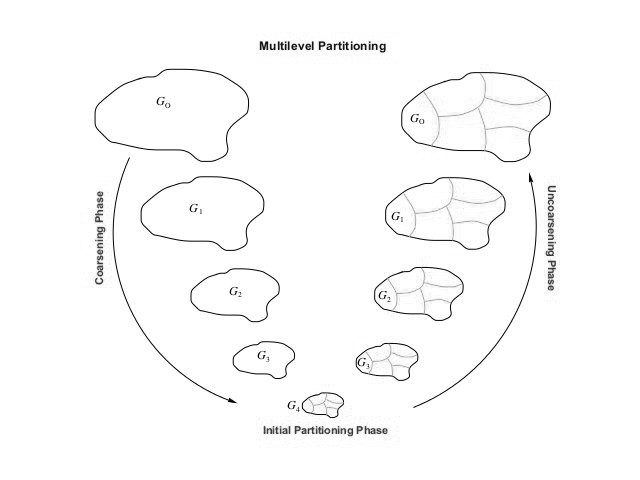
\includegraphics[scale=0.59]{Figures/metis.jpg}
	\rule{35em}{0.6pt}  % UnderLine figure	
    \caption[METIS-]{Οι τρεις φάσεις του multilevel k-way graph partitioning. Κατά την διάρκεια της συμπίεσης (coarsening), το μέγεθος του γράφου μειώνεται επιτυχώς.
    Κατά την διάρκεια του initial partitioning, υπολογίζεται ένα k-way partitioning. Κατά την διάρκεια της multilevel refinement (ή
    uncoarsening) φάσης, οι κατατμήσεις αποσυμπιέζονται διαδοχικά και προβάλλονται σε όλο και μεγαλύτερους γράφους. G0 είναι ο input γράφος, ο οποίος είναι ο λιγότερο συμπιεσμένος.
    Gi+1 είναι ο αμέσως πιο συμπιεσμένος γράφος και ο G4 είναι ο πιο συμπιεσμένος γράφος που θα υπάρξει. \cite{karypisΜetis}}
  \label{fig:metisFig}
  \end{center}
\end{figure}

    
Η ενσωμάτωση του Metis στον java κώδικα μας πραγματοποιείτε με τη χρήση της κλάσης Gpmetis \cite{GpMetis} της βιβλιοθήκης χειρισμού γράφων Grph,
η οποία αναλαμβάνει τη μεταγλώττιση (compile) του C κώδικα σε πραγματικό χρόνο, την εκτέλεση των διαδικασιών και τον χειρισμό του Ι/Ο.

